\chapter{Augmented Reality}

To help better the understanding of augmented reality, this chapter will describe the historical background as well as how it works. In section \ref{sec:ARtype} there
are a few different types of AR explained. Then a brief history of AR is presented in section \ref{sec:ARhistory}. Afterwards, a method about mapping the environment called \textit{S.L.A.M} is described in section \ref{sec:ARslam}. The chapter is rounded in section \ref{subsecARKit} with some information about how the the toolkit used in this project, \textit{ARKit}, functions. 

\section{The different types of Augmented Reality}
\label{sec:ARtype}
There are different types of augmented reality. Some of those are marker-based, location-based, superimposition-based and projection-based. \\

\textbf{Marker-based} AR is when markers, in the form of images have to be placed in the real world and detected by the application. Virtual object are rendered on top of these markers. An example would be a picture in a magazine which, when pointing a camera at it, the application renders a 3D object on top. An example is shown in figure \ref{fig:marker-based-ar} \\

\begin{figure}[hbtp]
\begin{center}
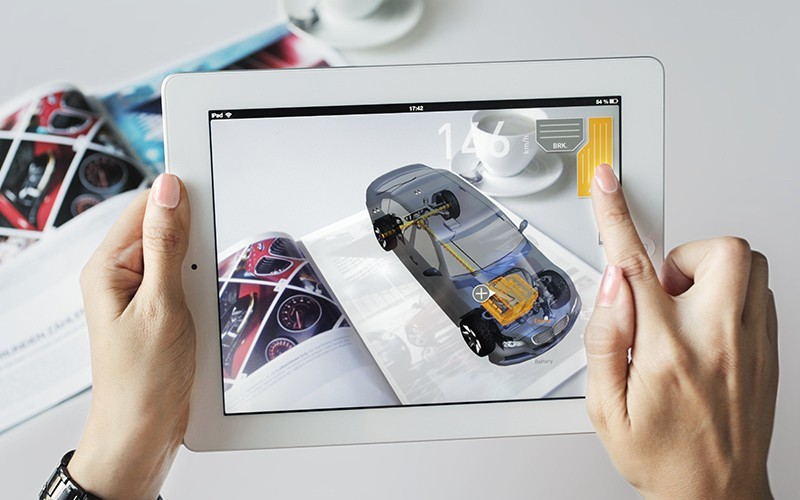
\includegraphics[width = 0.75\textwidth]{./Images/markerbasedar.jpg} 
\caption{A virtual object in the form of a car being rendered on top of a marker in a magazine.}
\label{fig:marker-based-ar}
\end{center}
\end{figure}

\textbf{Location-based} AR is when the content on the users screen differs depending on the location of the user. This type is highly dependent on the GPS signal.
An example of where this could be useful is in a museum where different information could be given to the user depending on which room he or she is in.\\

\textbf{Superimposition-based} AR uses object recognition in order to enhance that object with some sort of visual information. It replaces the real object with an enhanced virtual one. It could be used in retail to display different patterns on a piece of clothing.\\

\textbf{Projection-based} AR is when virtual object can be placed in a room to make it appear as if they were there. A popular example of this would be the IKEA Place app that was mentioned in the introduction. An example is shown in figure \ref{fig:projection-based-ar} \\

\begin{figure}[hbtp]
\begin{center}
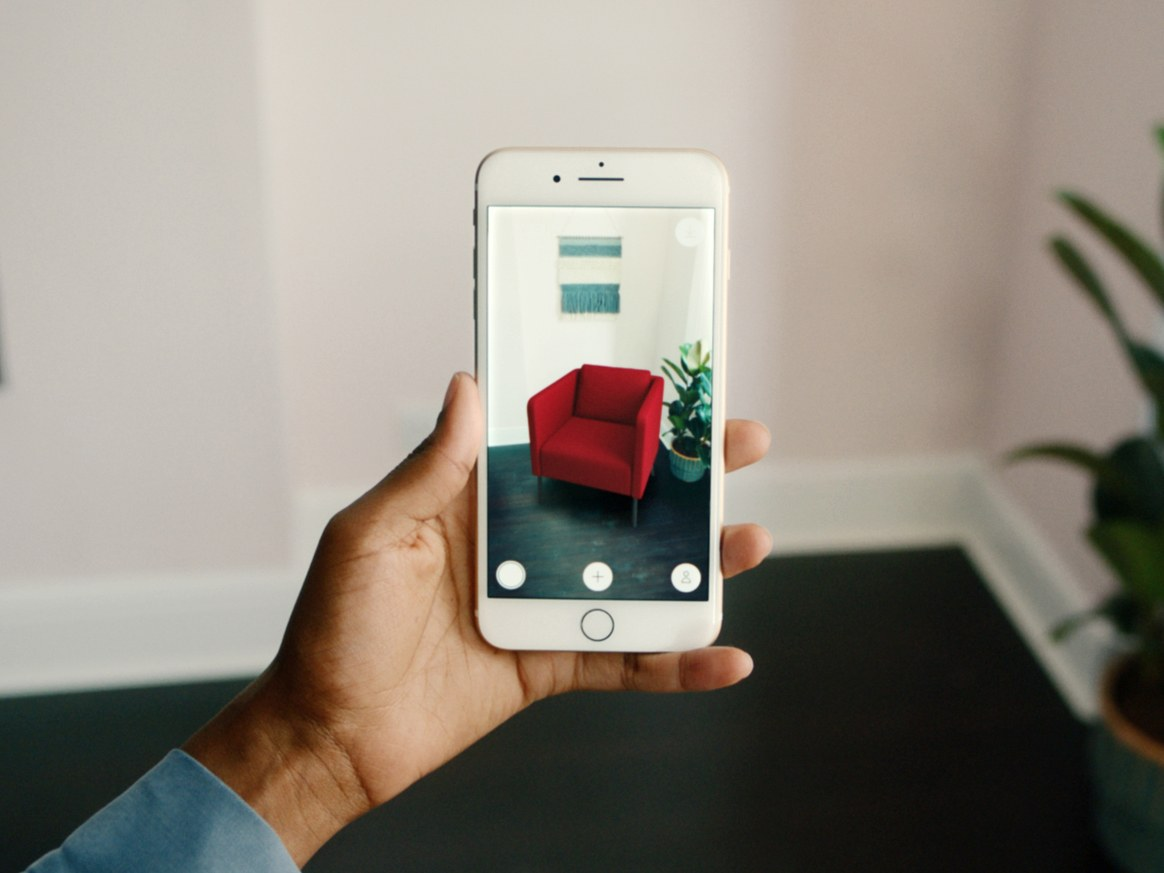
\includegraphics[width = 0.75\textwidth]{./Images/ikeaplace.jpg} 
\caption{A virtual sofa chair being added to a room within the IKEA Place app.}
\label{fig:projection-based-ar}
\end{center}
\end{figure}

In this paper we will mainly be using projection based AR with a form of recognition. The projections will be in the form of way-pointers used as instructions for the user to perform the next step in putting together a furniture piece. These instructions can visualize how the pieces will look like after the step is completed, and to show arrow pointers between the pieces that are supposed to be put together.

\section{History of AR}
\label{sec:ARhistory}
The idea of augmented reality has existed a long time, the phrase has only been used for about 30 years but it is not until recently that the technology has become mainstream.
This is mainly due to it becoming good enough to be used by the average person at home. Today we can just download an app on our smart phones to enjoy the technology. Below follows a brief history of how augmented reality has progressed throughout the years.\\

\textbf{1968}
The Sword of Damocles - The first mounted headset.
This device was mounted on the head and could display a cube wireframe floating in the air. It was invented by Ivan Sutherland.\\

\textbf{1975}
Myron Krueger - Videoplace. Using cameras to interact with a digital world with shadows.
This application could be used to draw things or play simple video games with the shadow of your hand.
\cite{videoplace}\\

\textbf{1990}
The first time the term "Augmented Reality" was used by the Boeing researcher Tom Caudell.\\

\textbf{2009}
AR comes to the web in the form of an open source toolkit called ARToolKit.\\

\textbf{2017}
Apple launches AR Kit and Google launches AR Core.\\

\section{S.L.A.M.}
\label{sec:ARslam}
S.L.A.M (Simultaneous Localization and Mapping) is a way for a machine to get to know the environment that it is in. It registers features and maps them to its surroundings. S.L.A.M is about having the map of the environment and knowing where the robot is in that map.
The problem with this is that a map is needed for knowing where you are, and you have to know where you are to be able to create a map. That is why S.L.A.M is doing this at the same time, hence 'Simultaneous'. The system is used in autonomous robots, but also valuable in Augmented Reality. \cite{slam}
In figure \ref{fig:slam} a robot is driving around in a room collecting data. The robots 
camera can be seen in the lower left corner. On the right, a 3D model with 
recognized feature points has been created.

iPhone X does this by tracking multiple reference points in space and from them building a 3D model of the surroundings using a form of S.L.A.M technique.
This is accomplished by keeping a map of the features while keeping track of the path the observer is taking. A number of 
hardware components make this task possible, including gyro, accelerometer and a compass. \cite{iphoneslam}

\begin{figure}[hbtp]
\begin{center}
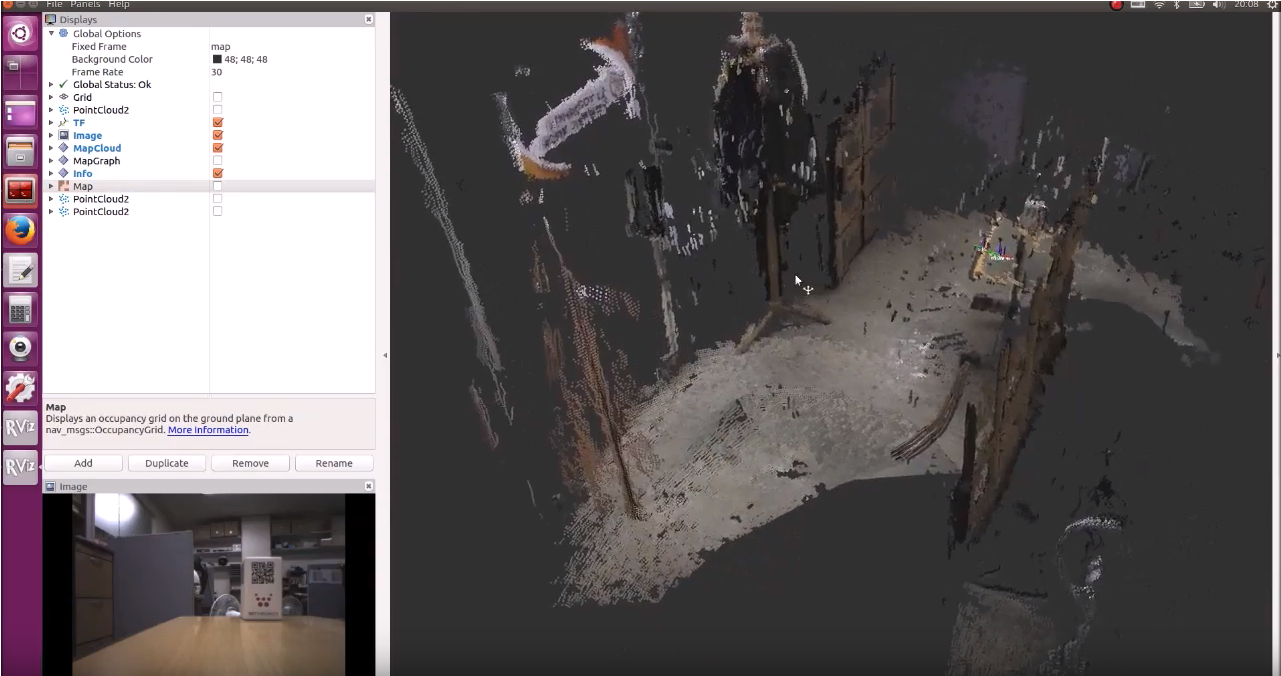
\includegraphics[width = 0.75\textwidth]{./Images/slam-map.jpg} 
\caption{A robot performing S.L.A.M in an environment and the 3D model created.}
\label{fig:slam}
\end{center}
\end{figure}

\section{How ARKit works}
\label{subsecARKit}
The easiest way to use ARKit is to use it through Xcode, which can be downloaded from the Mac App Store.
The coding language can be either Objective-C or Swift. We will be using Swift for all
examples.

ARKit works similar to SceneKit where a scene, which is basically a 3D environment in which nodes containing 3D models, known as geometries, can be rendered, is loaded at start up and interacted with.
An ARScene is contained inside an ARSCNView (AR Scene View) which also has an ARSession
that that manages the motion tracking and camera image processing. For an ARScene to work, it must have a running ARSession.
The session is started with configuration (ARConfiguration). This configuration can be of many kinds, the most common ones begin ARWorldTrackingConfiguration and ARFaceTrackingConfigurations. For this project, ARWorldTrackingConfiguration will be used since the face tracking one uses the front camera.

Below, an example of how to setup a configuration and running a session using Swift is given:

\begin{lstlisting}[language=swift]
func loadWorldTrackingConfiguration()
    {
        let configuration = ARWorldTrackingConfiguration()
        configuration.planeDetection = [.horizontal]

        // All the objects that are tracked is contained in the Objects folder
        guard let detectingObjects = ARReferenceObject.referenceObjects(inGroupNamed: "Objects", bundle: nil) else { return }
        configuration.detectionObjects = detectingObjects
        
        // Setting up tracking of images
        for imageURL in trackingImageURLs
        {
            guard let image: CGImage = UIImage(named: imageURL)?.cgImage else { return }
            let referenceImage = ARReferenceImage(image, orientation: CGImagePropertyOrientation.up, physicalWidth: 0.3)
            configuration.detectionImages.insert(referenceImage)
        }

        configuration.maximumNumberOfTrackedImages = trackingImageURLs.count
        
        // Running the sessoin with the configuration
        sceneView.session.run(configuration)
    }
\end{lstlisting}

But before a session can be started, an ARScene must exist and be loaded. The ARScene is a regular .scn file that has the starting nodes that together form the starting
environment the user will interact with. An example of how a scene like that looks like is shown in figure \ref{fig:3dsceneImage}.

\begin{figure}[hbtp]
\begin{center}
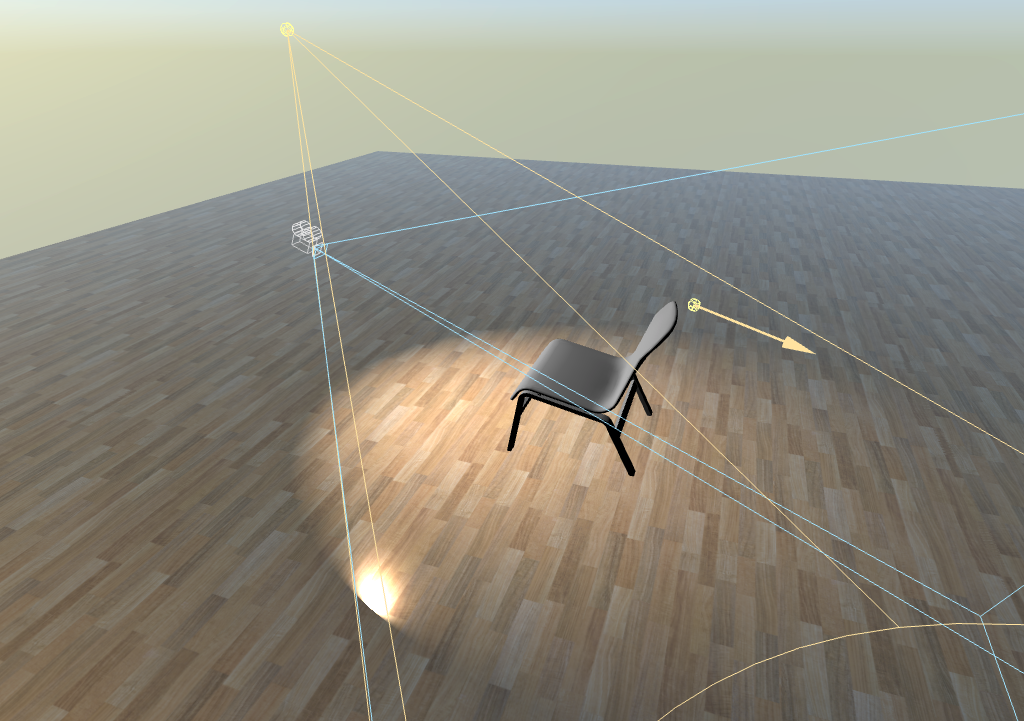
\includegraphics[width = 0.75\textwidth]{./Images/3dscene.jpg} 
\caption{An example of a 3D scene created in XCode with a camera, a plane, directional light and three geometry nodes.}
\label{fig:3dsceneImage}
\end{center}
\end{figure}

To load a scene, a new .scn file must be created in the art.scnassets folder and fetched like below.
\begin{lstlisting}[language=swift]
// Load the scene
let scene = SCNScene(named: "art.scnassets/world.scn")!        
sceneView.scene = scene
\end{lstlisting}

When ARScene detects objects, images, planes etc. it calls the renderer function. This function can be implemented by setting the ViewController to conform to the ARSCNViewDelegate. ARScene adds an anchor (ARAnchor) and a node (SCNNode) for the place where it detected it, and this can be used inside the function to render new nodes or other logic.

\begin{lstlisting}[language=swift]
func renderer(_ renderer: SCNSceneRenderer, didAdd node: SCNNode, for anchor: ARAnchor)
    {
    	    // If detected an object
        if let objectAnchor = anchor as? ARObjectAnchor
        {
        	   // Add some 3D text to the scene
            let objectName = objectAnchor.referenceObject.name!
            let textNode = GeometryFactory.makeText(text: objectName)
            node.addChildNode(textNode)
        }
        // If detected a plane
        else if let planeAnchor = anchor as? ARPlaneAnchor
        {
        // Add a plane geometry of the detected floor to the scene
        node.addChildNode(GeometryFactory.createPlane(planeAnchor: planeAnchor, metalDevice: metalDevice!))
            model.numberOfPlanesDetected += 1
        }
    }
\end{lstlisting}

If nodes need to be rendered outside of this function it can be done by accessing the
scenes root node.

\begin{lstlisting}[language=swift]
sceneView.scene.rootNode.addChildNode(node)
\end{lstlisting}


\newpage